\documentclass[protokol.tex]{subfiles}
\begin{document}
\begin{comment}
\begin{table}[H] \label{tab:podminky}
\centering
\setlength{\tabcolsep}{10pt}
\begin{tabular}{ccc}                                                    \toprule
Teplota                 &   Tlak                    &   Vlhkost     \\
$[\si{\degreeCelsius}]$ &   $[\si{\hecto\pascal}]$  &   [\% RH]     \\  \midrule
25,3                    &   984,5                   &   29,8        \\  \bottomrule
\end{tabular}
\caption{Podmínky měření}
\end{table}

\begin{figure}[H]
\centering
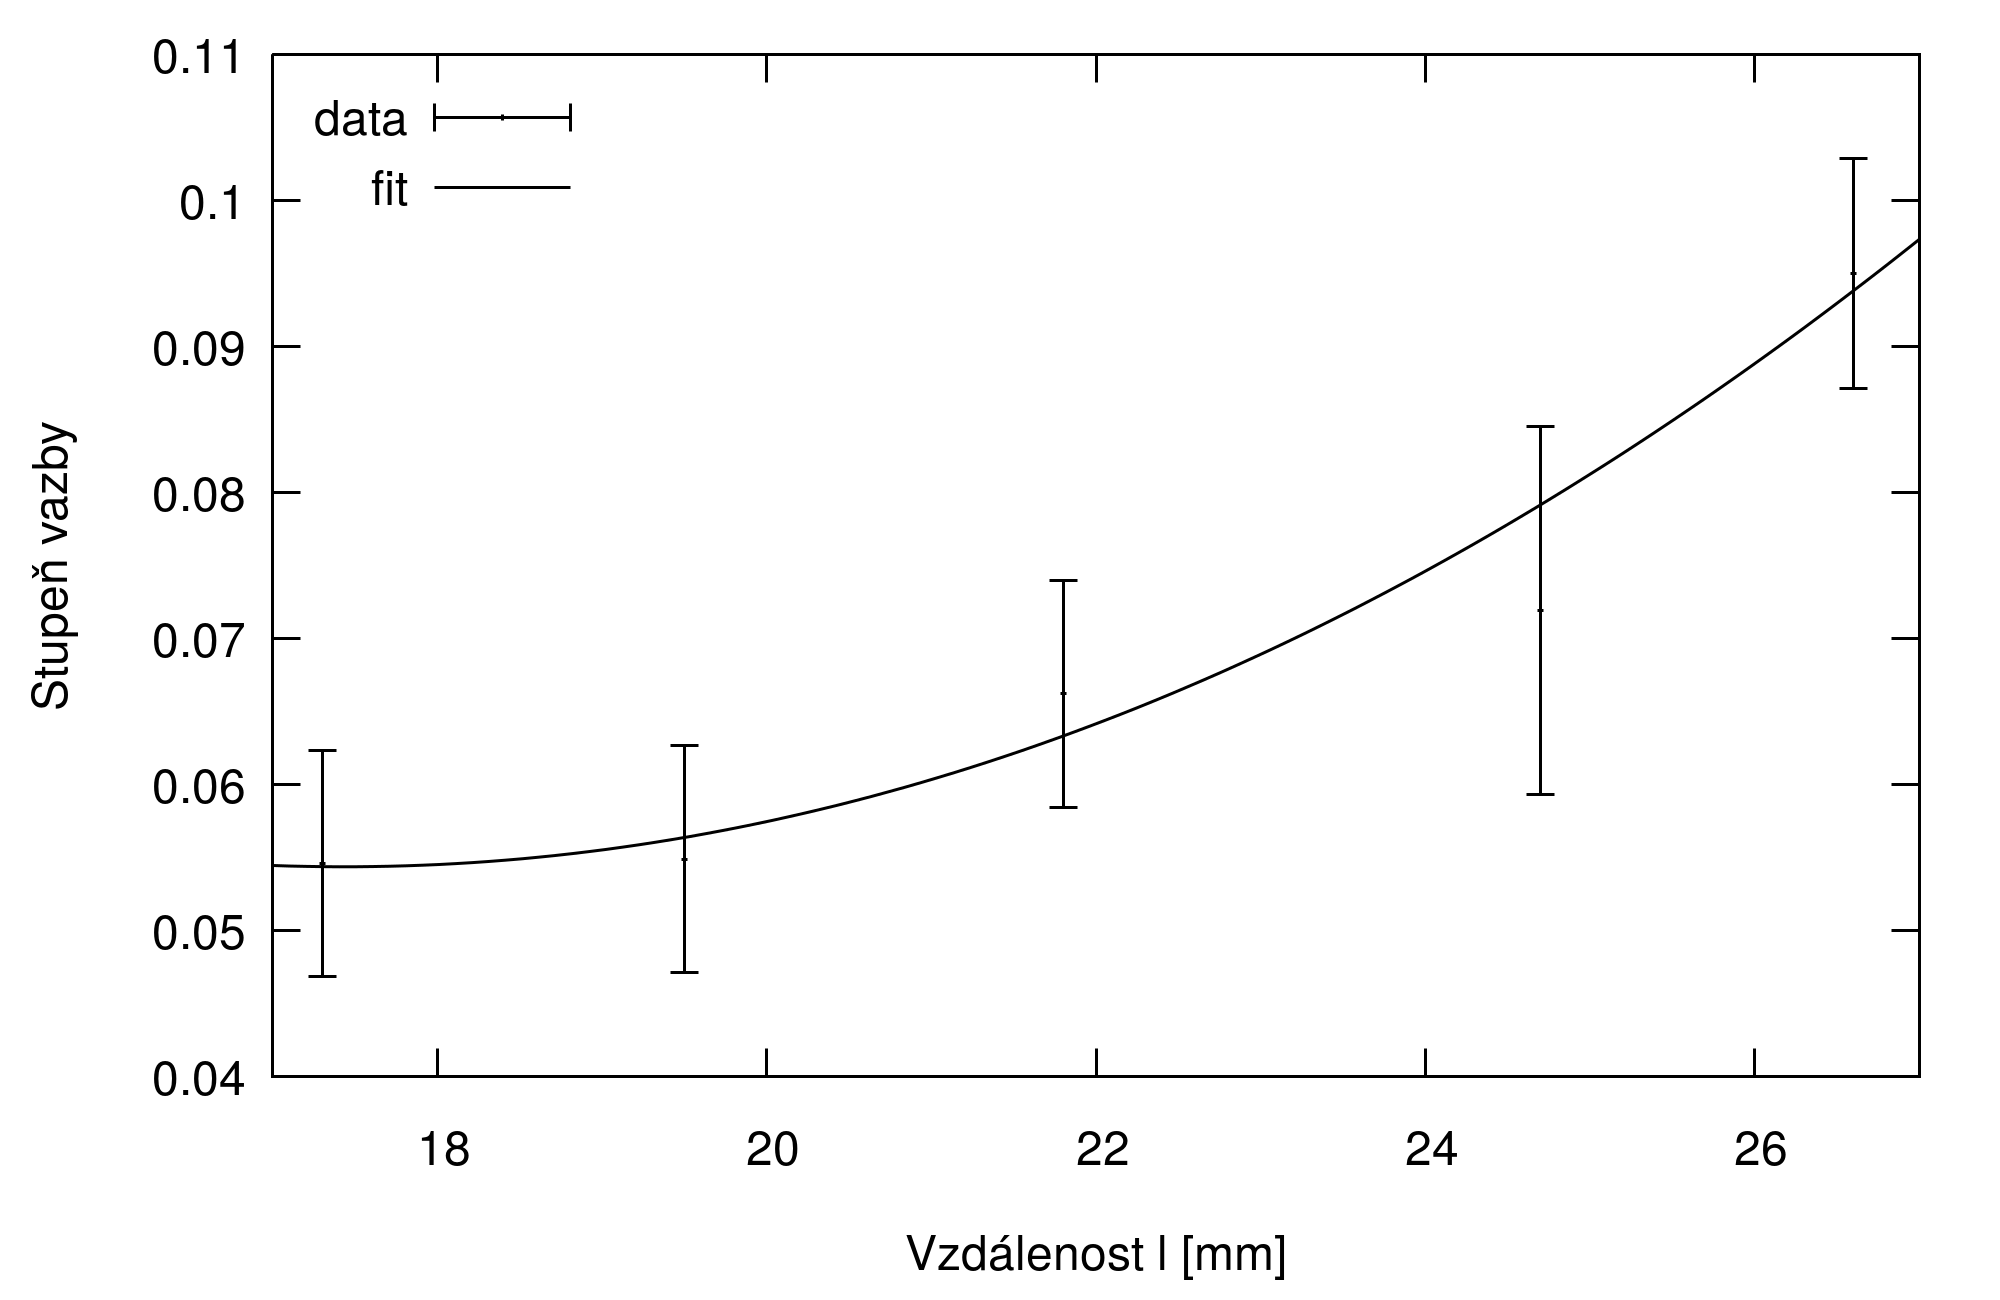
\includegraphics[resolution=350]{plot/graf}
\caption{Graf závislosti napětí na relativním prodloužení}
\end{figure}
\end{comment}

\begin{table}[H] \label{tab:podminky}
\centering
\setlength{\tabcolsep}{10pt}
\begin{tabular}{ccc}                                                    \toprule
Teplota                 &   Tlak                    &   Vlhkost     \\
$[\si{\degreeCelsius}]$ &   $[\si{\hecto\pascal}]$  &   [\% RH]     \\  \midrule
25,3                    &   984,5                   &   29,8        \\  \bottomrule
\end{tabular}
\caption{Podmínky měření}
\end{table}

\subsection*{Úkol 1}
Hmotnost závaží byla měřena na elektronických vahách.
$$ m = (148.0 \pm 0.1) \ \si{\gram} $$

Vzdálenost hmotného středu závaží od osy otáčení kola byla určena jako součet vzdálenosti hm. středu závaží od okraje tyče držící kolo a poloviny průměru této tyče. Z důvodu obtížného způsobu měření a nepřesnému odhadu polohy hmotného středu závaží kvůli jeho nedokonalého tvaru byla určena poměrně vysoká nejistota měření.
$$ l = (234 \pm 3) \ \si{\milli\metre} $$

Perioda kmitů byla měřena stopkami s ručním spouštěním. Naměřené hodnoty jsou uvedeny v následující tabulce.

\begin{table}[H] \label{tab:kyv}
\centering
\setlength{\tabcolsep}{8pt}
\begin{tabular}{cccccccccc}                                                                                                                          \toprule
                        &   1       &   2       &   3       &   4       &   5       &   průměr  &   $\sigma_{stat}$ &   $\sigma_{\text{měř}}$   &   $\sigma_{abs}$  \\  \midrule
$10 T [\si{\second}]$   &   24.54   &   24.52   &   24.43   &   24.43   &   24.45   &   24.474  &   0.023           &   0.01                    &   0.025           \\    
$   T [\si{\second}]$   &   2.454   &   2.452   &   2.443   &   2.443   &   2.445   &   2.4474  &   0.0023          &   0.001                   &   0.0025          \\  \bottomrule  
\end{tabular}
\caption{Perioda kyvu kola}
\end{table}

Podle \eqref{eq:kyv} je moment setrvačnosti kola 
$$ I = (0.0434 \pm 0.0005) \ \si{\kilo\gram\metre\squared} $$

\subsection*{Úkol 2}
Hmotnosti pěti závaží $A$ až $E$ byly naměřeny citlivými váhami. V experimentu k působení závaží přistupuje navíc proměnlivé působení vlákna, proto byla k naměřeným hodnotám přičtena polovina hmotnosti vlákna a výrazně zvýšena nejistota.
$$ m_A = (12.2 \pm 0.1) \ \si{\gram} $$
$$ m_B = (17.2 \pm 0.1) \ \si{\gram} $$
$$ m_C = (24.9 \pm 0.1) \ \si{\gram} $$
$$ m_D = (34.6 \pm 0.1) \ \si{\gram} $$
$$ m_E = (49.4 \pm 0.1) \ \si{\gram} $$  

Průměry souosých válců byly měřeny posuvným měřidlem, následně děleny dvěma.
$$ r_1 = (2.99 \pm 0.01) \ \si{\milli\metre} $$
$$ r_2 = (4.98 \pm 0.01) \ \si{\milli\metre} $$
$$ r_3 = (6.97 \pm 0.01) \ \si{\milli\metre} $$
$$ r_4 = (8.94 \pm 0.01) \ \si{\milli\metre} $$

\newpage

Následující graf znázorňuje závislost úhlové rychlosti na čase pro tři různé konfigurace (hodnoty $r$ a $m$).
\begin{figure}[H]
\centering
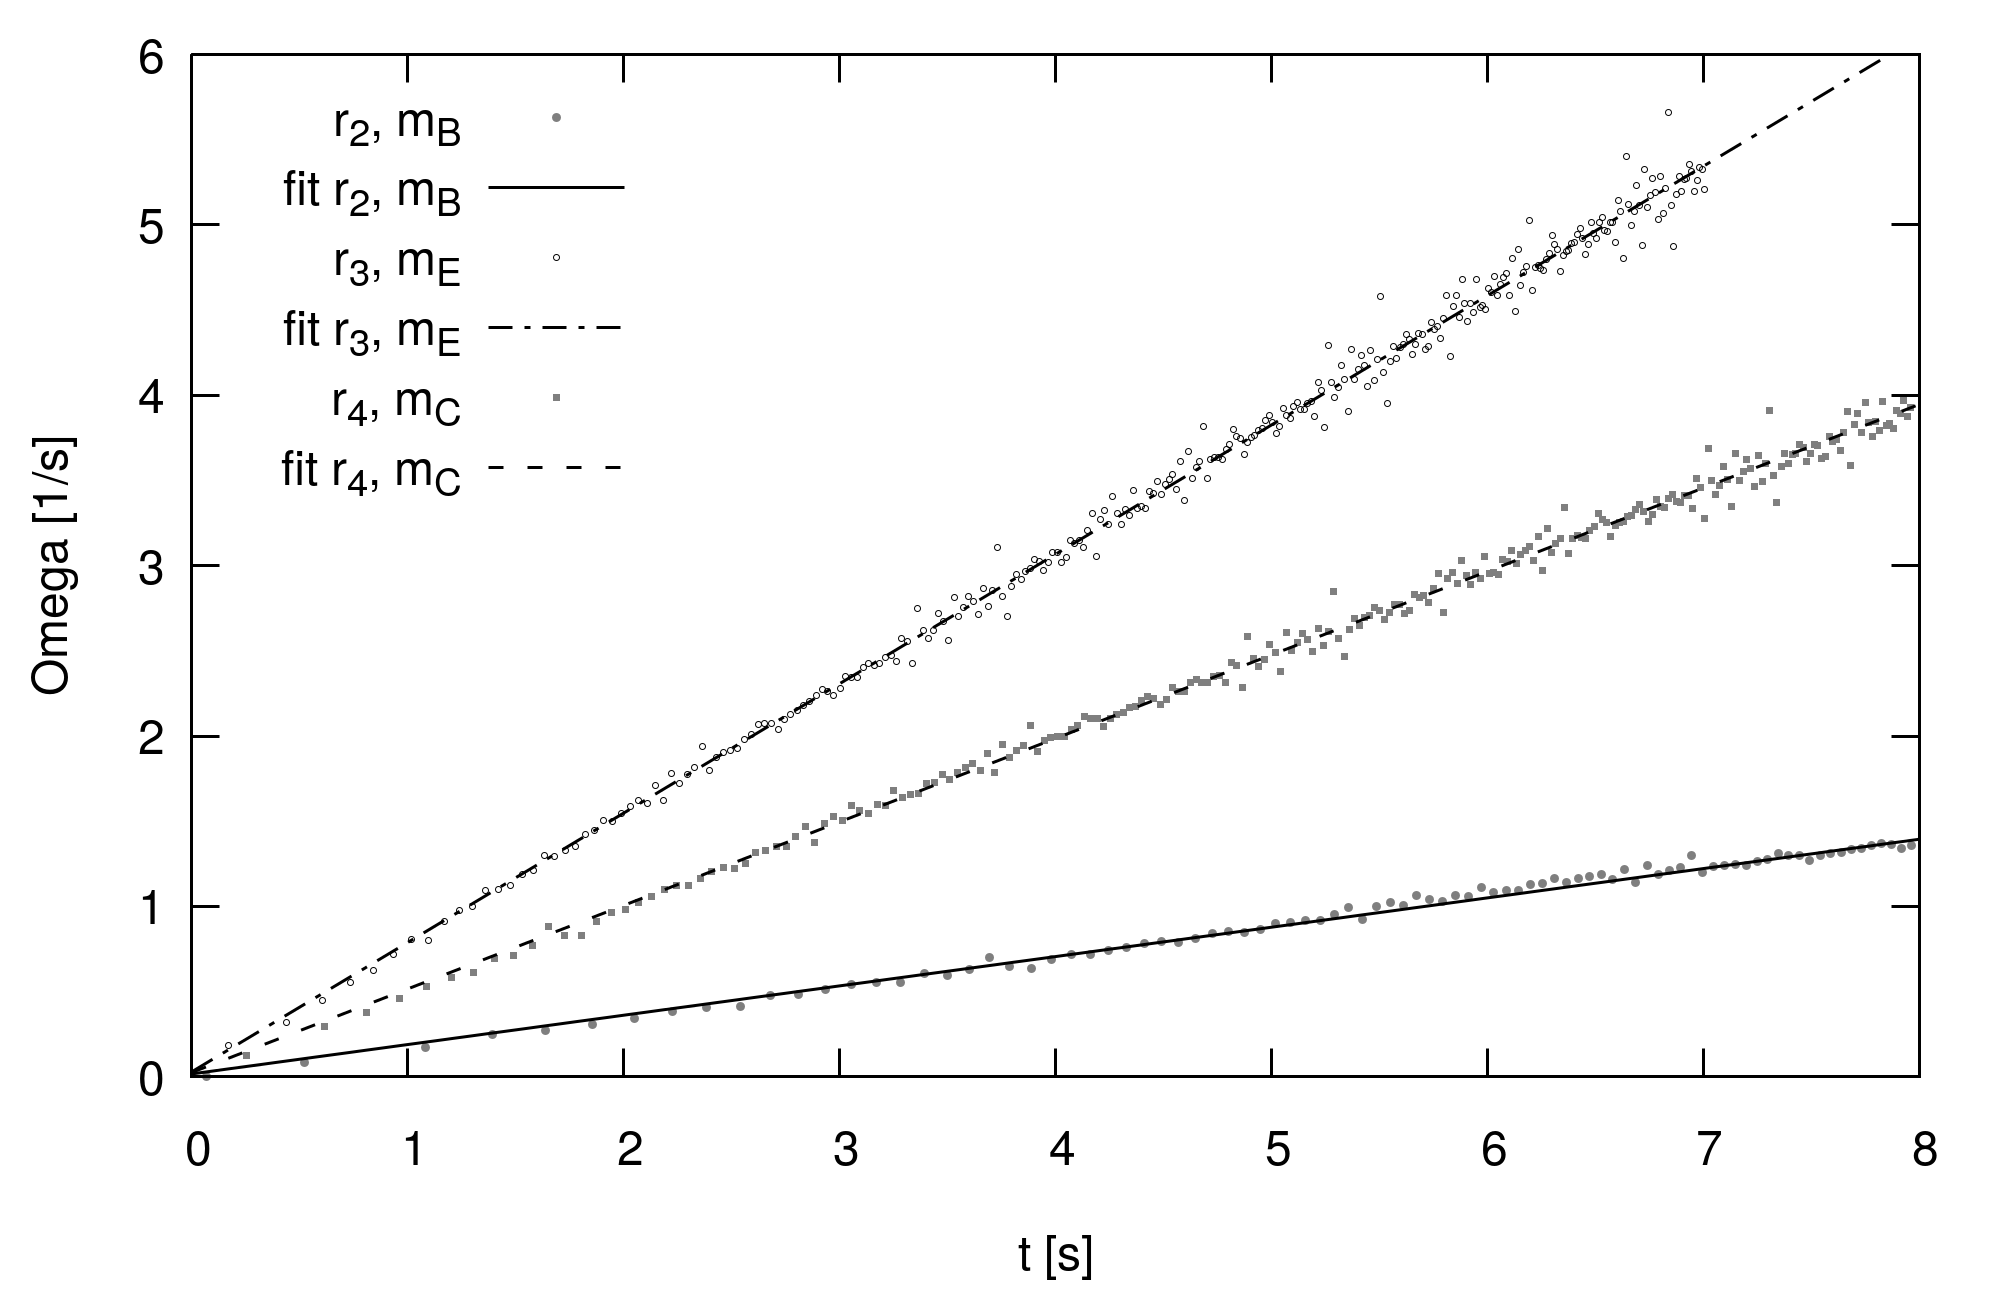
\includegraphics[resolution=350]{plot/out}
\caption{Závislost $\omega$ na $t$ pro konfigurace $r_2$, $m_B$; $r_3$, $m_E$ a $r_4$, $m_C$}
\end{figure}

Lineárním fitem dostaneme 
$$ \epsilon_{2B} = (0.1721 \pm 0.0007) $$
$$ \epsilon_{3E} = (0.759  \pm 0.003 ) $$
$$ \epsilon_{4C} = (0.490  \pm 0.002 ) $$

\newpage

\subsection*{Úkol 3 a 4}
Následující graf zachycuje závislost $I^*$ na parametru $\alpha$ podle vztahu \eqref{eq:nekorig_na_alpha}.
\begin{figure}[H]
\centering
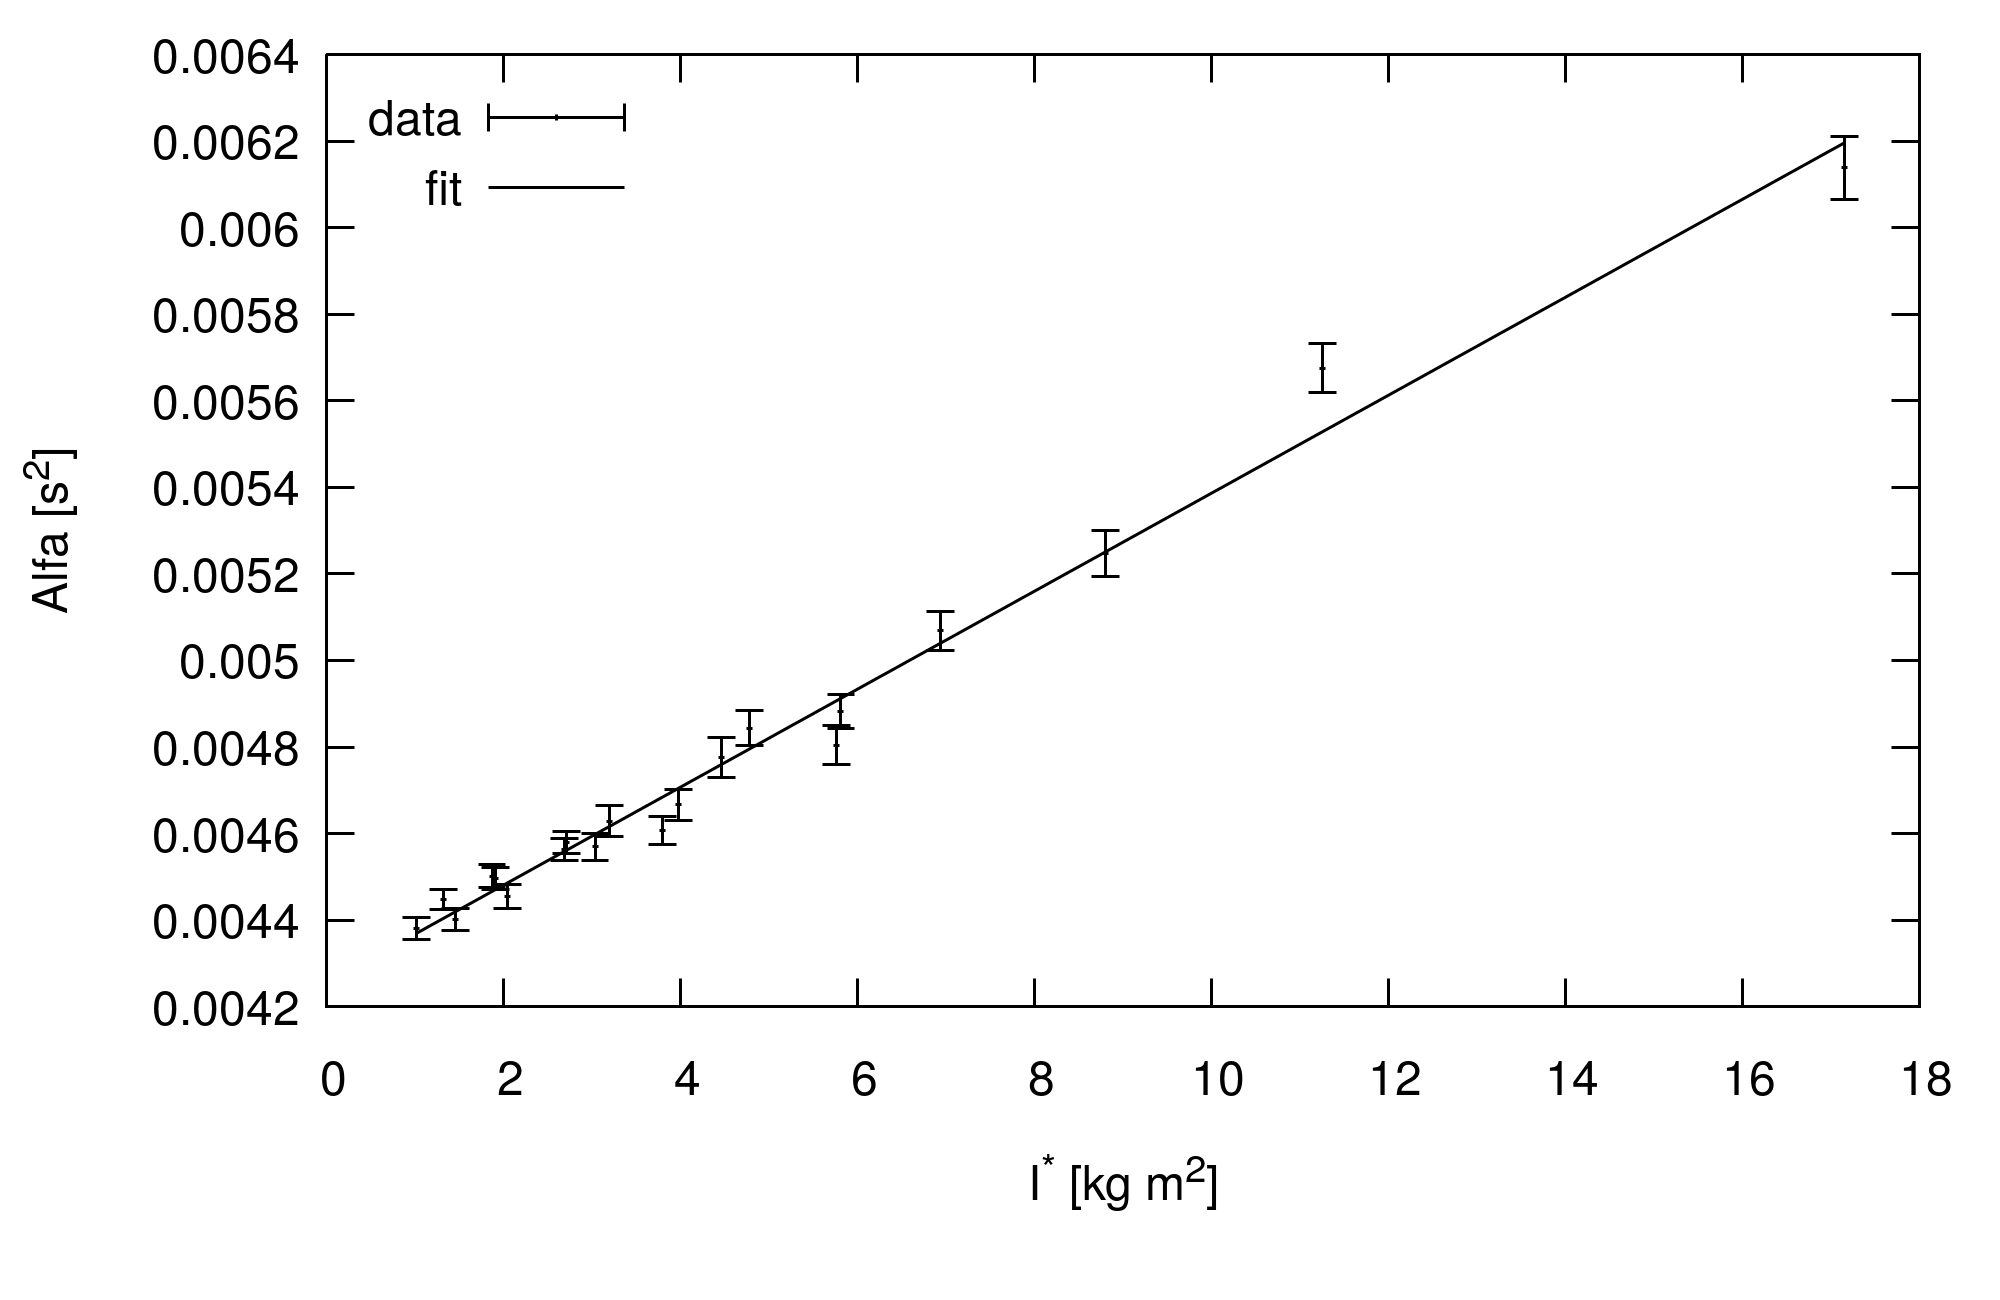
\includegraphics[resolution=350]{plot/IaM.png}
\caption{Závislost $I^*$ na $\alpha$}
\end{figure}

Lineární regresí získáme
$$ M_T = (0.113 \pm 0.003) \times \num{e-3} \ \si{\newton\metre} $$
$$ I_k = (0.00425 \pm 0.00005) \ \si{\kilo\gram\metre\squared} $$

\end{document}
